%proposed replacement for discussion

%\kjx{could be two subsetions or one section}

%\subsection{Examplars}

The design of \Chainmail was guided by the study of a sequence of
exemplars taken from the object-capability literature and the smart
contracts world:

\begin{enumerate}
\item \textbf{Bank} \cite{arnd18} - Bank and accounts as described in
Section~\ref{sect:motivate:Bank}, with two different implementations given in Appendix~\ref{Bank:appendix}
\item
\textbf{ERC20} \cite{ERC20} - Ethereum-based token contract
\item
\textbf{DAO} \cite{Dao,DaoBug} - Ethereum contract for Decentralised Autonomous
Organisation
\item
\textbf{DOM} \cite{dd,ddd} - Restricting access to browser Domain Object Model\\
\end{enumerate}\vspace{-1em}

\subsection{Authorising ERC20}
\label{sect:example:ERC20}
{ 
 ERC20~\cite{ERC20} is a widely used token standard which describes the 
 basic functionality expected by any    Ethereum-based token contract. 
 It issues and keeps track of participants' tokens, and supports the  transfer
 of tokens between participants. 
%
%
%An important question, therefore, is to identify the precise circumstances under which a transfer of tokens may take place.
%The answer is that 
Transfer of tokens 
 can   take place only provided that  there were sufficient tokens in the
 owner's account, and that
 the transfer was instigated by the owner, or by somebody authorized
 by the owner.

We specify this in \Chainmail as follows:
A decrease in  a participant's \prg{balance} 
%(\ie  $\prg{e}.\prg{balance}=...\, \wedge\, \Next{\prg{e}.\prg{balance}=...}$)
can only be caused by a transfer instigated by the 
account holder themselves\\ (\ie $\Calls {\prg{p}} {\prg{transfer}} {...} {...}$), or by
an authorized transfer instigated by another participant $\prg{p}''$  (\ie $\Calls {\prg{p}''} {{\prg{transferFrom}} } {..} {..}$) who 
has authority for more than the tokens spent (\ie  $\prg{e}.\prg{allowed}(\prg{p},\prg{p}'')\geq \prg{m}$)
 
\vspace{.15cm}
\noindent
% \strut \hspace{0.3cm} 
$\forall \prg{e}:\prg{ERC20}.\forall \prg{p}:\prg{Object}.\forall \prg{m},\prg{m}':\prg{Nat}.$\\
\strut \hspace{0.3cm} $[\ \ \prg{e}.\prg{balance(p)}=\prg{m}+\prg{m'}\ \wedge \ \Next{\prg{e}.\prg{balance(p)}=\prg{m}'}$ \\ %.\forall\prg{m}:\prg{Nat}.$\\
\strut \hspace{0.4cm} \ \ \ $\longrightarrow$\\
\strut \hspace{0.4cm} \ \ \ $\exists \prg{p}',\prg{p}'':\prg{Object}.$ \\
\strut \hspace{0.4cm} \ \ \  $[\ \  \Calls{\prg{p}} {\prg{transfer}}  {\prg{e}}  {\prg{p}',\prg{m}} \  \  \ \vee\, $\\
\strut \hspace{0.4cm} \ \ \   $\ \ \ \ \prg{e}.\prg{allowed}(\prg{p},\prg{p}'')\geq \prg{m} \ \wedge \ \Calls{\prg{p}''} {\prg{transferFrom}}  {\prg{e}}  {\prg{p}',\prg{m}}\       \  ]$\\
\strut \hspace{0.3cm} $] $
\vspace{.15cm}

\noindent
That is to say: if next configuration witnesses a decrease of \prg{p}'s balance by
 $\prg{m}$, then the current configuration was a call of \prg{transfer} instigated by
 \prg{p}, or  a call of \prg{transferFrom} instigated by somebody authorized by \prg{p}.
 The term $\prg{e}.\prg{allowed}(\prg{p},\prg{p}'')$,  means that the
ERC20 variable \prg{e} holds a field called \prg{allowed}   which maps pairs of participants to numbers; such
mappings are supported in Solidity\cite{Solidity}.
 
We now define what it means for $\prg{p}'$ to be authorized  to  spend 
up to \prg{m} tokens on  $\prg{p}$'s behalf: At some point in the
past,  \prg{p} gave authority to $\prg{p}'$  to spend   \prg{m}
plus the sum of  tokens
spent so far by $\prg{p}' $ on the behalf of \prg{p}. 

 
\vspace{.15cm}
\noindent
 $\forall \prg{e}:\prg{ERC20}.\forall \prg{p},\prg{p'}:\prg{Object}.\forall \prg{m}:\prg{Nat}.$\\
\strut \hspace{0.3cm} $[\ \ \prg{e}.\prg{allowed}(\prg{p},\prg{p}')=\prg{m} $\\
\strut \hspace{0.4cm} \ \ \ $\longrightarrow$\\
\strut \hspace{0.4cm} \ \ \  
     $\PrevId\langle\ \  \Calls{\prg{p}}  {\prg{approve}}  {\prg{e}} {\prg{p}',\prg{m}} $\\
      \strut \hspace{1.7cm} \ $\vee $\\
\strut \hspace{1.7cm} \  
     $    \prg{e}.\prg{allowed}(\prg{p},\prg{p}')=\prg{m}   
        \  \wedge\ $\\
\strut \hspace{1.5cm} \ \ \ \ \          
$  \neg   (\, {\Calls{\prg{p}'} {\prg{transferFrom}} {\prg{e}} {\prg{p},\_}   } \, \vee \, {\Calls{\prg{p}} {\prg{approve}} {\prg{e}} {\prg{p},\_} } \, ) $\\
      \strut \hspace{1.7cm}\  $\vee $\\
\strut \hspace{1.7cm}   \  $ \exists \prg{p}'':\prg{Object}.\exists\prg{m'}:\prg{Nat}.$\\
 \strut \hspace{1.7cm}\  $[\   
  \prg{e}.\prg{allowed}(\prg{p},\prg{p}')=\prg{m}+\prg{m}'  \, \wedge\,   {\Calls{\prg{p}'} {\prg{transferFrom}} {\prg{e}} {\prg{p}'',\prg{m}'}  }   ]$\\
\strut \hspace{0.4cm} \ \ \  \ \ \  \ \ \ \ \ $\rangle $\\
\strut \hspace{0.3cm} $]$
\vspace{.15cm}
 
In more detail\  $\prg{p}'$ is allowed to spend 
up to \prg{m} tokens on their behalf of $\prg{p}$, if in the   previous step either a)
 \prg{p} made the call \prg{approve} on \prg{e} 
with arguments $\prg{p}'$ and \prg{m}, or b)  
$\prg{p}'$ was allowed to spend  up to \prg{m} tokens for $\prg{p}$
and did not transfer any of \prg{p}'s tokens, nor did \prg{p} issue a fresh authorization,
or c) \prg{p} was authorized for $\prg{m}+\prg{m}'$ and spent $\prg{m}'$. 
  
  \vspace{.1cm}
 
 Thus, the holistic specification gives to account holders an
 "authorization-guarantee": their balance cannot decrease unless they
 themselves, or somebody they had authorized, instigates a transfer of
 tokens. Moreover, authorization is {\em not} transitive: only the
 account holder can authorise some other party to transfer funds from
 their account: authorisation to spend from an account does not confer
 the ability to authorise yet more others to spend also.
 
% \paragraph{Comparison with Traditional Specifications}
 
 With traditional  specifications, to obtain the "authorization-guarantee", 
one would need to inspect the pre- and post- conditions of {\em all} the functions
in the contract, and determine which of the functions decrease balances, and which of the functions 
 affect authorizations.
 In the case of the \prg{ERC20}, one would have to inspect all eight such specifications
 (given in appendix \ref{ERC20:appendix}), 
 where only five are relevant to the question at hand.
 In the general case, \eg the DAO, the number of   functions which are unrelated
 to the question at hand can be very large.
  
More importantly, with traditional  specifications, nothing stops the next release of the contract to add, 
\eg, a method which allows participants to share their authority, and thus
violate the "authorization-guarantee", or even a super-user from skimming 0.1\% from each of the accounts.

}

\subsubsection{ERC20, the traditional specification}
\label{ERC20:cont}
We compare the holistic and the traditional specification of ERC20.

As we said earlier,  the holistic specification gives to account holders an
 "authorisation-guarantee": their balance cannot decrease unless they
 themselves, or somebody they had authorised, instigates a transfer of
 tokens. Moreover, authorisation is {\em not} transitive: only the
 account holder can authorise some other party to transfer funds from
 their account: authorisation to spend from an account does not confer
 the ability to authorise yet more others to spend also.
 
 With traditional  specifications, such as is shown in appendix~\ref{sect:ERC20:appendix}, to obtain the "authorisation-guarantee", 
one would need to inspect the pre- and post-conditions of {\em all} the functions
in the contract, and determine which of the functions decrease balances, and which of the functions 
 affect authorisations.
In Figure \ref{fig:classicalERC20} we outline a traditional specification for the \prg{ERC20}.
We give two specifications for \prg{transfer}, another two for \prg{tranferFrom}, and one for all 
the remaining functions. The  first specification says, \eg, that if  
 \prg{p} has sufficient tokens, and it calls \prg{transfer}, then the transfer will take place.  
The second specification says that  if \prg{p} has insufficient tokens, then 
the transfer will not take place (we assume that in this
specification language, any entities not mentioned in the pre- or post-condition 
are not affected).
 
 Similarly, we would have to give another two specifications to define the behaviour of 
if \prg{p''} is authorised and executes \prg{transferFrom}, then   the balance decreases. 
But they are {\em implicit} about the overall behaviour and the   {\em necessary} conditions,
e.g., what are all the possible actions that can cause a decrease of balance?



\subsection{Defending the DAO}
\label{Dao:appendix}
The DAO  {(Decentralised Autonomous Organisation)}~\cite{Dao}  is a famous Ethereum contract  which aims to support
collective management of funds,  and to place power directly in the
hands of the owners of the DAO
rather than delegate it to directors.
Unfortunately, the DAO was not robust:
a re-entrancy bug   exploited in June 2016 led  to a loss of   \$50M, and
a hard-fork in the  chain ~\cite{DaoBug}.
%
%In a similar style as that  of the ERC20 spec earlier,
%We can give a \Chainmail~specification
With holistic specifications  we can  write a succinct requirement that a
DAO contract should always be able to repay any owner's money.
Any contract which satisfies such a holistic specification cannot demonstrate the DAO bug.
 
Our specification consists of three requirements.
First, that the DAO always holds at least as 
much money as any owner's balance.
%  \james{ALL owners? or does that follow?} 
To express this we use 
the field \prg{balances} which is a mapping from participant's addresses to 
numbers. Such mapping-valued fields exist in Solidity, but they could
also be taken to be ghost fields~\cite{ghost}.
  
\vspace{.1cm}

\noindent
 \strut \hspace{0.5cm} $\forall \prg{d}:\prg{DAO}.\forall \prg{p}:\prg{Any}.\forall\prg{m}:\prg{Nat}.$\\
\strut \hspace{0.5cm} $[\ \ \prg{d.balances(p)}=\prg{m}  \ \ \  \longrightarrow  \ \ \ \prg{d}.\prg{ether}\geq \prg{m} \ \ ] $


\noindent
Second, that when an owner asks to be repaid, she is sent all her money.
\vspace{.1cm}

\noindent
 \strut \hspace{0.5cm} $\forall \prg{d}:\prg{DAO}.\forall \prg{p}:\prg{Any}.\forall\prg{m}:\prg{Nat}.$\\
\strut \hspace{0.5cm} $[\ \ \prg{d.balance(p)}=\prg{m}
 \ \wedge \ \Calls{\prg{p}}{\prg{repay}}{\prg{d}}{\_}  $\\
 $\strut \hspace{5.5cm}   \ \ \  \longrightarrow  \ \ \  \Future{\Calls{\prg{d}}{\prg{send}}{\prg{p}}{\prg{m}}}\ \ ] $  
\vspace{.1cm}

 

%\kjx{combined defn ensuring enough eth at the time repayment is made:\\
%\noindent
% \strut \hspace{0.5cm} $\forall \prg{d}:\prg{DAO}.\forall \prg{p}:\prg{Any}.\forall\prg{m}:\prg{Nat}.$\\
%\strut \hspace{0.5cm} $[\ \ \prg{d.balance(p)}=\prg{m}
% \ \wedge \ \Calls{\prg{p}}{\prg{repay}}{\prg{d}}{\_}  $\\
% $\strut \hspace{5.5cm}   \ \ \  \longrightarrow  \ \ \  \Future{\Calls{\prg{d}}{\prg{send}}{\prg{p}}{\prg{m}}
% \wedge \prg{d}.\prg{ether}\geq \prg{m}}\ \ ] $
%\vspace{.1cm}
%}
%
%\kjx{negative example for talk, upping funds not calling send:\\
%\noindent
% \strut \hspace{0.5cm} $\forall \prg{d}:\prg{DAO}.\forall \prg{p}:\prg{Any}.\forall\prg{m}:\prg{Nat}.$\\
%\strut \hspace{0.5cm} $\ \ \Calls{\prg{d}}{\prg{send}}{\prg{p}}{\prg{m}}
% \strut \ \ \  \longrightarrow  \ \ \  \prg{d}.\prg{ether}\geq \prg{m}$\\
% % SD thinks the last  \longrightarrow sgould be wedge
%  $\strut \ \ \  \longrightarrow  \ \ \  \prg{p.funds}
%  = \Prev{\prg{p.funds}} + \prg{m}$
%\vspace{.1cm}
%}


\noindent
\sd{Third, that the balance of an owner is a function of its balance in the previous step,
or the result of it joining the DAO, or asking to be repaid \etc.}
 
\noindent
$\strut \hspace{0.5cm} \forall \prg{d}:\prg{DAO}.\forall \prg{p}.\forall:\prg{m}:\prg{Nat}.$\\
$\strut \hspace{0.5cm} [ \ \ \  \prg{d.Balance(p)}=\prg{m} \ \ \  \longrightarrow   
 \ \  \ \ 
  [ \  \ \Prev{\Calls{\prg{p}}{\prg{repay}}{\prg{d}}{\_}}\, \wedge\, \prg{m}=\prg{0} \ \ \ \ \vee $\\
$\strut \hspace{5.7cm}      
\Prev{\Calls{\prg{p}}{\prg{join}}{\prg{d}}{\prg{m}}}  \ \ \ \ \vee   $\\
 $\strut \hspace{5.7cm}  ... \  ]$ \\
%                         
%                         $ \left\{
%                            \begin{array}{ll}
%                             \prg{0}, & \hbox{if}\ Prev(Call(\prg{p},\prg{d.repay(),\_})    \\
%                             \vee
%                             \\
%                             \prg{m},  & \hbox{if}\  Prev(Call(\prg{p},\prg{d.join(),m}))   \\
%                             ..., & ...
%                           \end{array}
%                         \right.    $\\
$\strut \hspace{0.5cm} ] $
  


More cases are needed to reflect the financing and repayments of proposals, but they can be expressed with the concepts described so far.


 

\noindent
The requirement that \prg{d} holds at least \prg{m} ether precludes the DAO bug,
in the sense that  any contract satisfying that spec cannot exhibit  the  bug:   a contract
which satisfies the spec  is guaranteed to always have enough money to satisfy all \prg{repay} requests.
This guarantee  holds, regardless of how many functions there are in the DAO.
In contrast, to preclude the DAO  bug with a classical spec, one would need to write a spec for each of the
DAO functions (currently 19), a spec for each function of the auxiliary contracts used by the DAO,
and then study their emergent  behaviour.

These 19 DAO functions   have several different concerns:
who may vote   for a proposal, who is eligible to submit a proposal,
how long the consultation period is for deliberating a proposal, what
is the quorum, how to chose curators, what is the value of a token,
Of these groups of functions, only  a handful affect the balance of a
participant. Holistic specifications allow us to concentrate on aspect of DAO's behaviour across \emph{all} its functions.
 


\subsection{Attenuating the DOM}
\label{sect:example:DOM}
%We will now discuss  an example demonstrating the need to describe attenuation in specifications.
\emph{Attenuation} is the ability to provide to third party objects \emph{restricted}  access to an object's functionality. This is usually achieved through the introduction of an intermediate object. While such intermediate objects are a common programming practice, 
the term was coined, and the practice  was studied in detail in the object capabilities literature,
e.g.  \cite{MillerPhD}. 

The key structure underlying a web browser is the Domain Object Model
(DOM), a recursive composite tree structure of objects that represent
everything displayed in a browser window.  Each window has a single DOM
tree which includes both the page's main content and also third party
content such as advertisements. To ensure third party content cannot
affect a page's main content,
specifications for attenuation for the DOM were proposed in
\textit{Devriese et al:}   \cite{dd}. 
%In this section we revisit that example and also argue that compared with the specification in \cite{dd}, our specification xxxx.

This example deals with a tree of DOM nodes: Access to a DOM node
gives access to all its parent and children nodes, and the ability to
modify the node's properties. However, as the top nodes of the tree
usually contain privileged information, while the lower nodes contain
less crucial third-party information, we want to be able to limit  access given to third parties to only the lower part of the DOM tree. We do this through a \prg{Wrapper}, which has a field \prg{node} pointing to a \prg{Node}, and a field \prg{height} which restricts the range of \prg{Node}s which may be modified through the use of the particular \prg{Wrapper}. Namely, when you hold a \prg{Wrapper}  you can modify the \prg{property} of all the descendants of the    \prg{height}-th ancestors of the \prg{node} of that particular \prg{Wrapper}. % It is not difficult to write such a \prg{Wrapper}; a possible implementation  appears in Figure \ref{fig:DOM} in appendix \ref{DOM:traditional}.


In Figure \ref{fig:WrapperUse} we show an example of the use of  \prg{Wrapper} objects attenuating the use of \prg{Node}s  The function \prg{usingWrappers} takes as parameter an object of unknown provenance, here called \prg{unknwn}. On lines 2-7 we create  a tree consisting of nodes \prg{n1}, \prg{n2}, ... \prg{n6}, depicted as blue circles on the   right-hand-side of the Figure. On line 8 we create a wrapper of \prg{n5} with height \prg{1}. This means that the wrapper \prg{w} may be used to modify \prg{n3}, \prg{n5} and \prg{n6} (\ie the objects in the green triangle), while it cannot be used to modify \prg{n1}, \prg{n2}, and \prg{4} (\ie the objects within the blue triangle). 
On line 8 we call a  function named \prg{untrusted} on the \prg{unknown} object, and pass \prg{w} as   argument. 

\begin{figure}[htb]
\begin{tabular}{llll}
\ \ &
\begin{minipage}{0.45\textwidth}
\begin{lstlisting}
method usingWrappers(unknwn){
   n1=Node(null,"fixed"); 
   n2=Node(n1,"robust"); 
   n3=Node(n2,"const"); 
   n4=Node(n3,"volatile");
   n5=Node(n4,"variable");
   n6=Node(n5,"ethereal");
   w=Wrapper(n5,1);
   
   unknwn.untrusted(w);
   
   assert n2.property=="robust" 
   ...
}
\end{lstlisting}
\end{minipage}
& & 
\begin{minipage}{0.75\textwidth}
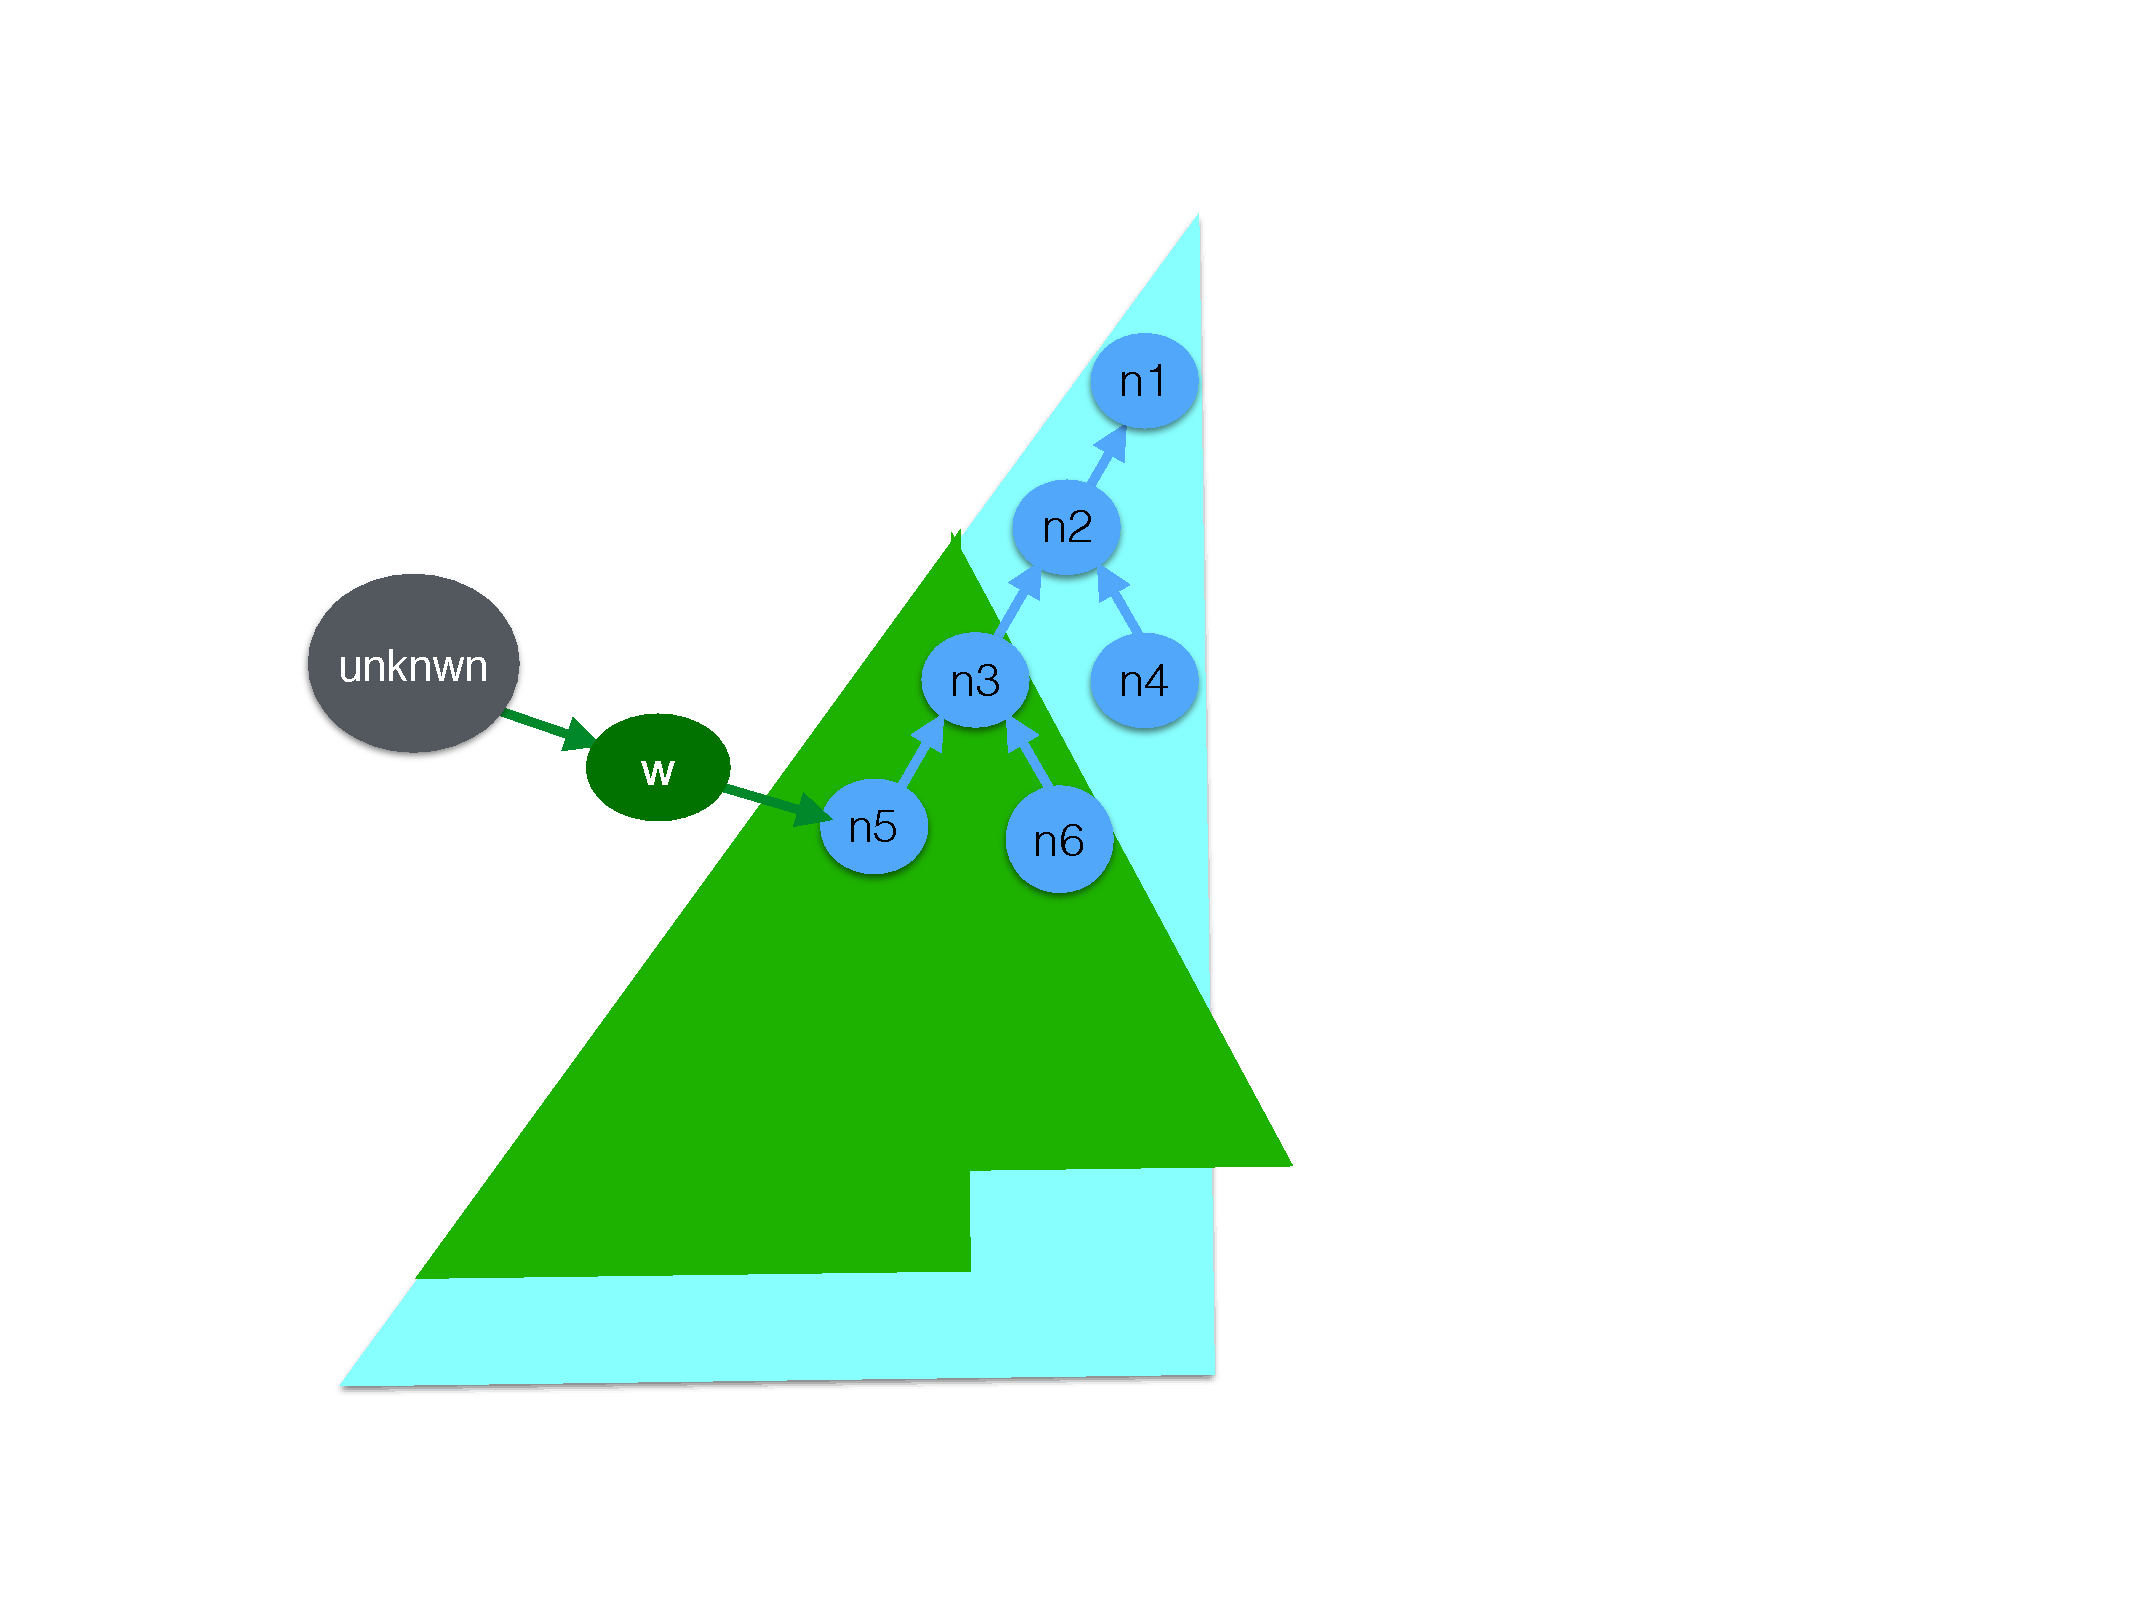
\includegraphics[width=\linewidth, trim=145  320 60 105,clip]{diagrams/DOM.pdf}
% x y z w
% y seems to eat up the bollom
% y=320 is good
% x eats space from left, if you increase it the diagram decreases from left
% w eats space from top, if you increase it the diagram decreases from top
% w=100 is good
%\includegraphics[page=3, width=\linewidth, trim=150  270 40 150, clip]{diagrams/snmalloc.pdf}\sdcomment{I think we need to change the diagram so that it says small slab.}
\strut \\
\strut \\

\end{minipage}
\end{tabular}
 \vspace*{-4.5mm}
\caption{\prg{Wrapper}s protecting \prg{Node}s }
\Description{A node labelled unknown, pointing to the node labelled ``w'' for ``wrapper'', and six nodes in a triangular area, labelled n1 through n6. The triangular area is bisected, the lower half is green and the upper half is blue. Nodes n3, n5, and n6 lie in the green half. nodes n4, n2, and n1 in the blue half. n1 has child n2, n2 has children n3 and n4, and n3 has children n5 and n6.}
\label{fig:WrapperUse}
\end{figure}

Even though we know nothing about the \prg{unknown} object or its \prg{untrusted} function, and even though the call gives to \prg{unknown}  access to \prg{w}, which in turn has transitive access to all  \prg{Node}-s in the tree, 
we know that %the call to the \prg{untrusted} function is guaranteed not to 
line 100 will not affect the   \prg{property} fields of the nodes \prg{n1}, \prg{n2}, and \prg{n4}. 
Thus, the assertion on line 12 is guaranteed to succeed. 
The question is how do we specify \prg{Wrapper}, so as to be able to make such an argument. %prove this assertion.

A  specification of the class \prg{Wrapper} 
in the traditional   style, \eg  \cite{Leavens-etal07} %(\cf appendix \ref{DOM:traditional}) 
consists of pairs of pre- and post- conditions for each of the
functions of that class. Each such pair gives a {\em sufficient}
condition for some effect to take place: for example the
call \prg{w.setProperty(i,prp)} where \prg{i} is smaller
than \prg{w.height} is a sufficient condition to
modify   \prg{property} of the \prg{i}-th parent of \prg{w.node}. But
we do not know what other ways there may be  to modify a
node's  \prg{property}. In other words, we have not specified
the \emph{necessary conditions}.
%
%\footnote{Shell we say the following, or does it break the flow? \\
%Moreover, on line 10 we do not know which functions are called on \prg{w}.}
%
%Instead, in this work, we propose \emph{holistic specifications},
%which describe the behaviour of an abstract data type as a hole,
%taking all possible method calls into account. Such holistic
%specifications typically describe \emph{necessary conditions} for some
%effect to take place.
%
In our example:

\begin{quote}
The \emph{necessary} condition for the modification of \prg{nd.property} for some \prg{nd} of class \prg{Node}  is either access to some   \prg{Node} in the same tree, or  access to a \prg{w} of class \prg{Wrapper} where the \prg{w.height}-th parent of \prg{w} is an ancestor of \prg{nd}.
\end{quote}


With such a specification we can prove that the assertion on line 12 will succeed. And, more importantly, we can ensure that all future updates of the \prg{Wrapper} abstract data type will uphold the \emph{protection} of the \prg{Node} data.
%
% Having justified the need for  necessary conditions in specifications, 
%
To give a flavour of \Chainmail, we use it  express the requirement from above:
%  This  gives us the opportunity to  demonstrate primitives for time ($\Future{\_}$) and authority ($\Changes{\_}$ and $\Using {\_} {\_}$).
 % and   more traditional relations between objects ( $\prg{nd}.\prg{parnt}^k\!=\! ...$):
% $\strut$ 
\vspace{.1cm}

\noindent
% \begin{quote}
$\forall \prg{S}:\prg{Set}.\forall \prg{nd}:\prg{Node}.\forall \prg{o}:\prg{Object}.$\\
$[$ \\
$\strut\  \ {\Using{\Future {\Changes {\prg{nd.property}}}}  {\prg{S}}}$ \\
$\strut  \ \ \longrightarrow$\\
$\strut \ \ \ \exists \prg{o}.[\ \prg{o}\in\prg{S}\ \ \wedge\ \ \neg(\prg{o}:\prg{Node})\ \ \wedge\  \ \neg(\prg{o}:\prg{Wrapper})\ \ \ \wedge \  $\\
$ \strut\ \ \  \ \ \ \ \ \ \ \ [\ \exists \prg{nd}':\prg{Node}. \CanAccess{\prg{o}}{\prg{nd}'}\  \ \ \  \vee$\\
$ \strut\ \  \ \  \ \  \ \ \ \ \ \ \ \exists \prg{w}:\prg{Wrapper}.\exists k\!:\!\mathbb{N}.
% $\\ $ \strut \ \ \ \ \ \ \ \ \ \ \ \ \ \ \ \ \  \ \ \
  (\ \CanAccess{\prg{o}}{\prg{w}}  \ \wedge\ \prg{nd}.\prg{parnt}^k\!=\!\prg{w.node}.\prg{parnt}^{\prg{w.height}}) \ \ \ ]\ ]$\\
$ ]$
% \end{quote}

\vspace{.1cm}

%\kjx{edited for talk:\\
%\noindent
%% \begin{quote}
%$\forall \prg{S}:\prg{Set}.\forall \prg{nd}:\prg{Node}.\forall \prg{o}:\prg{Object}.$\\
%$[\ \ {\Using{\Future {\Changes {\prg{nd.property}}}}  {\prg{S}}}$ \\
%$\strut  \ \ \longrightarrow$\\
%$\strut \ \ \ \exists \prg{o}.[\ \prg{o}\in\prg{S}\ \ \wedge\ \ \neg(\prg{o}:\prg{Node})\ \ \wedge\  \ \neg(\prg{o}:\prg{Wrapper})\ \ \ \wedge \  $\\
%$ \strut\ \ \ \ \ [\ \exists \prg{nd}':\prg{Node}. \CanAccess{\prg{o}}{\prg{nd}'}\  \ \ \  \vee$\\
%$ \strut\ \  \ \  \ \  \ \ \exists \prg{w}:\prg{Wrapper}.\exists k\!:\!\mathbb{N}.
%  (\ \CanAccess{\prg{o}}{\prg{w}}$\\
% $ \strut \ \ \ \ \ \ \ \ \  \ \ \
%\ \wedge\ \prg{nd}.\prg{prnt}^k\!$\\
% $ \strut \ \ \ \ \ \ \ \ \ \ \ \ \  \ \ \
%=\!\prg{w.node}.\prg{prnt}^{\prg{w.hgt}}) \ \ \ ]\ ]$\\
%$ ]$
%% \end{quote}
%}
%\vspace{.1cm}

\noindent
That is, if  the value of \prg{nd.property} is modified ($\Changes{\_}$) at some future point ($\Future{\_}$) 
and if reaching that future point involves no more objects than those from
set \prg{S} (\ie ${\Using{\_} {\prg{S}}}$), then at least one (\prg{o}) of the objects in \prg{S} is not a \prg{Node} nor a \prg{Wrapper}, and \prg{o} has direct access to some  node ($\CanAccess{\prg{o}}{\prg{nd}'}$), or  to some wrapper \prg{w} and the \prg{w.height}-th parent of \prg{w} is an ancestor of \prg{nd} (that is, $\prg{parnt}^k\!=\!\prg{w.node}.\prg{parnt}^{\prg{w.height}}$).
% It is important to clarify what we mean by ``access''. 
%Definitions of these concepts   appear later (Definition \ref{def:valid:assertion}), but  note
 Note that our ``access'' is intransitive: $\CanAccess x y$ holds if  either \prg{x} has a field  pointing to \prg{y}, or  \prg{x}  is the receiver and \prg{y} is one of the arguments  in the executing method call.
 
%% In the next sections we proceed with a formal model of our model. In the appendix we discuss more -- and simpler -- examples.
%% We chose the DOM for the introduction, in order to give a flavour of the \Chainmail features.
 


\subsection{Safe}
\label{sect:exampleSafe}
An earlier publication of this work, published at FASE 2020 \cite{FASE}, used an example of a Safe to
demonstrate how holistic specifications could be used to protect against dangerous implementations
of a safe. We now revisit this example, and discuss a bug that has since been discovered, along with
the nuance that this example points to in Chainmail. 

 \begin{figure}[htb]
 \begin{tabular}{lll} % {lll}
\begin{minipage}{0.45\textwidth}
\begin{lstlisting}
class Safe{
   field treasure 
   field secret 
   method take(scr){
      if (secret==scr) then {
         t=treasure
         treasure = null
         return t }  }
 }
\end{lstlisting}
\end{minipage}
  &\ \ \  \ \ \ \ \  \ \ \ \ \ \ &
\begin{minipage}{0.45\textwidth}
\begin{lstlisting}
class Safe{
   field treasure   
   field secret  
   method take(scr){
       $\mathit{... as\, version\,1 ...}$ 
   }
   method set(scr){
         secret=scr }
 }
\end{lstlisting}
\end{minipage} 
 \end{tabular}
  \vspace*{-0.95cm}
  \caption{Two Versions of the class \prg{Safe}}
 \label{fig:ExampleSafe}
 \vspace*{-0.65cm}
 \end{figure}

Consider the two implementations of a \prg{Safe} class in Figure \ref{fig:ExampleSafe}. Both implementations 
present a class with two fields:
\begin{itemize}
\item
\prg{treasure} : the object stored in the safe,  and 
\item
\prg{secret} : the password required to open the \prg{Safe} and remove the treasure.
\end{itemize}
Both implementations also include a method for using the 
 \prg{secret} to remove the \prg{treasure}: \prg{take}.
The second implementation also includes another method, \prg{set}, that allows any object to change the \prg{secret}.
This clearly violates any reasonable specification for a \prg{Safe}, and seems an ideal target for a Holistic specification.
 A classical Hoare triple describing the behaviour of \prg{take} would be:
 
  \vspace{.1in}
  
% \begin{figure}[htbp] 
(ClassicSpec)$  \ \ $  $\triangleq$
\vspace{-.1in}
\begin{lstlisting}
   method take(scr)
   PRE:   this:Safe  
   POST:  scr=this.secret$\pre$  $\longrightarrow$ this.treasure=null 
               $\wedge$
          scr$\neq$this.secret$\pre$ $\longrightarrow$  $\forall$s:Safe.$\,$s.treasure=s.treasure$\pre$
 \end{lstlisting}
%^\end{figure} 
\vspace{-.2in}

(ClassicSpec)  expresses  that knowledge of the \prg{secret} is  \emph{sufficient} %condition 
to remove the treasure, and further that  knowledge of the \prg{secret} is \emph{necessary} for
 \prg{take} to remove the \prg{treasure}. (ClassicSpec) does not however ensure that there
 is not some other means of removing the \prg{treasure}, or in the case of the second implementation
 of \prg{Safe}, changing the \prg{secret}. In order to capture such a specification, we would need 
 a holistic specification.
 
 
 
\vspace{.1in}
(HolisticSpec)\ \  $\triangleq$\\ 
$\strut \hspace{.3in}   \forall \prg{s}. % $\\ 
[\ \ \prg{s}:\prg{Safe} \wedge \prg{s.treasure}\neq\prg{null}   \wedge   \Future{\prg{s.treasure}=\prg{null}} $ \\ 
 $ \strut \hspace{4.3cm}     \longrightarrow \ \  \exists \prg{o}. [\  \External{\prg{o}} \wedge  \CanAccess{\prg{o}}{\prg{s.secret}}\ ]  \  \ ] \hfill $
\vspace{.1in}

(HolisticSpec) requires that for any \prg{Safe} with a non-null \prg{treasure}, if
that treasure is ever removed, it follows that there is some current external object 
with knowledge of the \prg{secret}. i.e. it is not possible to either forge, steal, 
or illegally modify the \prg{secret}. 

Both classes in Fig. \ref{fig:ExampleSafe} satisfy (ClassicSpec), and in the paper presented at FASE 2020 \cite{FASE}, 
we claimed that the first version satisfies (HolisticSpec) while the second does not. In fact neither implementation satisfies 
(HolisticSpec). The nuance is found in the notion of \prg{external} and \prg{internal}. The counter example to (HolisticSpec)
is where the \prg{secret} of one \prg{Safe}, say \prg{s1}, is stored as the \prg{treasure} of another, say \prg{s2}: i.e. \prg{s2.treasure = s1.secret}. 
In such a case, there might be no external objects with explicit knowledge of \prg{s1.secret} (since \prg{s2} is a \prg{Safe}, and thus considered \prg{internal}), but some object might 
know \prg{s2.secret}, and thus have a way to obtain \prg{s1.secret}, and finally removing \prg{s1.treasure}. 

The discovery of this bug identifies the nuances of \prg{external} and \prg{internal}. In the current formulation of 
Chainmail, these concepts are defined at a module level, but in the example of the Safe, are needed to be defined 
at a data-structure level. i.e. in our example above, we need to be able to say that \prg{s2} is external to \prg{s1}.
We have since reformulated the Safe example by making use of ghost fields to define what is internal and external 
to a \prg{Safe}.

 \begin{figure}[htb]
\begin{lstlisting}
class Safe{
   ghost is_internal(x) = x == this || x == secret
   field treasure 
   field secret 
   method take(scr){
      if (secret==scr) then {
         t=treasure
         treasure = null
         return t }  }
 }
\end{lstlisting}
  \vspace*{-0.95cm}
  \caption{A fixed version of the class \prg{Safe}}
 \label{fig:ExampleSafeFix}
 \vspace*{-0.65cm}
 \end{figure}

